\باب{سمتیات}
\حصہ{مقداری اور سمتیہ}
وہ طبعی مقدار جس کو اپنے مکمل اظہار کے لئے سمت کی ضرورت نہیں ہوتی \موٹا{مقداری}\فرہنگ{مقداری}\حاشیہب{scalar}\فرہنگ{scalar} کہلاتا ہے۔کسی چیز کی کمیت \عددیء{m} یا اس کا درجہ حرارت \عددیء{T} مقداری کی مثالیں ہیں۔مقداری کی قیمت اٹل یا متغیر ممکن ہے۔کمیت اٹل مقداری کی مثال ہے۔متغیر مقداری کی قیمت مختلف اوقات اور نقاط پر مختلف ہو سکتی ہے۔یوں کسی بھی نقطے پر درجہ حرارت کی قیمت وقت \عددیء{t} کے ساتھ تبدیل ہو سکتی ہے۔اسی طرح کسی بھی وقت مختلف نقاط پر درجہ حرارت کی قیمت مختلف ہو سکتی ہے۔یوں اگر صبح  کے وقت اسلام آباد میں کسی مقام پر درجہ حرارت \عددیء{\SI{12}{ \celsius}} ہو تو دوپہر کو اسی مقام پر درجہ حرارت \عددیء{\SI{30}{ \celsius}} ہو سکتا ہے۔درجہ حرارت \عددیء{T}، وقت \عددیء{t}،  \موٹا{کارتیسی محدد}\فرہنگ{کارتیسی محدد}\حاشیہب{Cartesian coordinates}\فرہنگ{Cartesian coordinates} کے متغیرات  \عددیء{x}، \عددیء{y} اور \عددیء{z} تمام مقداری متغیرات ہیں۔

ایسی طبعی مقدار جسے بیان کرنے کے لئے سمت درکار ہو \موٹا{سمتیہ}\فرہنگ{سمتیہ}\حاشیہب{vector}\فرہنگ{vector} کہلاتا ہے۔اس کتاب میں سمتیہ کی قیمت کو مثبت تصور کیا جائے گا۔یوں سمتیہ کی حتمی قیمت ہی اس کی مقدار ہو گی۔قوت، سمتی رفتار اور سمتی اسراع سمتیہ کی مثالیں ہیں۔

اس کتاب میں مقداری متغیرات کو سادہ طرز کی لکھائی میں انگریزی یا لاطینی زبان کے  چھوٹے حروف مثلاً \عددیء{a}، \عددیء{b}، \عددیء{\alpha}،\نقطے 
  یا بڑے حروف مثلاً \عددیء{A}، \عددیء{B}، \عددیء{\Psi}، \نقطے  سے ظاہر کیا جائے گا۔سمتیہ متغیرات کو موٹی لکھائی میں انگریزی یا لاطینی زبان کے  چھوٹے  یا بڑے حروف  سے ظاہر کیا جائے گا۔یوں قوت  کو \سمتیہ{F} جبکہ سمتی رفتار کو \سمتیہ{v} سے ظاہر کیا جائے گا۔قلم و کاغذ استعمال کرتے ہوئے سمتیہ پر تیر  یا آدھے تیر کا نشان بنایا جاتا ہے یوں قوت کو \عددیء{\vec{F}} یا  
$\overset{\rightharpoonup}{\rule{0pt}{.9ex}\smash{F}}$
لکھا جاتا ہے۔سمتیہ کو تیر سے ظاہر کیا جاتا ہے جہاں تیر کی لمبائی سمتیہ کی حتمی قیمت $\abs{\bf{F}}$  ظاہر کرتی ہے جبکہ سمتیہ کی سمت تیر کی سمت  سے ظاہر کی جاتی ہے۔سمتیہ کی حتمی قیمت کو سمتیہ ظاہر کرنے والے حرف کو چھوٹی لکھائی میں لکھ کر ظاہر کیا جاتا ہے۔یوں قوت \سمتیہ{F}  کی حتمی قیمت  کو \عددیء{F} لکھا جائے گا۔ 

شکل \حوالہ{شکل_سمتیہ_دم_پر_عمل_درامد_ہوتی_ہے} میں نقطہ \عددیء{(1,1)} پر پانی کی رفتار کو سمتیہ \سمتیہ{v} سے ظاہر کیا گیا ہے۔اس نقطے پر مثبت افقی محور کی سمت میں پانی کی رفتار \عددیء{\SI{2.5}{\meter \per \second}} ہے۔سمتیہ کی دُم اس مقام پر رکھی جاتی ہے جہاں سمتیہ کی قیمت بیان کی جا رہی ہو۔یوں شکل میں سمتیہ کی دُم  \عددیء{(1,1)} پر رکھی گئی ہے۔اس شکل میں \عددیء{\SI{1}{\centi \meter}} کی لمبائی \عددیء{\SI{1}{\meter \per \second}} کی رفتار کو ظاہر کرتی ہے۔
\begin{figure}
\centering
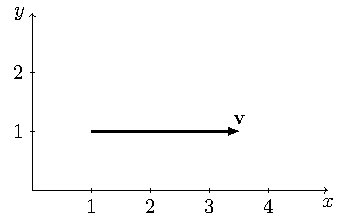
\includegraphics{vectorBaseAtPointOfAction}
\caption{سمتیہ}
\label{شکل_سمتیہ_دم_پر_عمل_درامد_ہوتی_ہے}
\end{figure}

\حصہ{سمتی الجبرا}
دو سمتیوں کا ترسیمی  مجموعہ حاصل کرنے کی خاطر ایک سمتیہ کے سر کو دوسری سمتیہ کے دُم  کے ساتھ ملایا جاتا ہے۔پہلی سمتیہ کی دُم سے دوسری سمتیہ کے سر تک سمتیہ حاصل جمع ہو گا۔اس عمل کو شکل \حوالہ{شکل_سمتیہ_سمتیوں_کا_مجموعہ}-الف میں دکھایا گیا ہے۔شکل میں \سمتیہ{A} کے سر کے ساتھ \سمتیہ{B} کی دُم ملائی گئی ہے۔دو سے زیادہ سمتیوں کا مجموعہ بھی اسی عمل کو استعمال کرتے  ہوئے حاصل کیا جاتا ہے۔اس عمل کو سر سے دُم جوڑنا\فرہنگ{سر سے دُم جوڑنا}\فرہنگ{head to tail rule}\حاشیہب{head to tail rule} کہتے ہیں۔شکل \حوالہ{شکل_سمتیہ_سمتیوں_کا_مجموعہ}-ب میں دو سمتیوں کے دُم ملا کر سمتیوں کے متوازی الاضلاع\فرہنگ{متوازی الاضلاع}\حاشیہب{parallelogram law}\فرہنگ{parallelogram law}  سے ان کا مجموعہ حاصل کرنا دکھایا گیا ہے جسے دیکھ کر صاف ظاہر ہے کہ $\bf{A}+\bf{B}=\bf{B}+\bf{A}$ ہے یعنی سمتیوں کا مجموعہ قانون تبادل\فرہنگ{قانون تبادل}\حاشیہب{commutative law}\فرہنگ{commutative law} پر پورا اترتا ہے۔اسی طرح سمتیوں کا مجموعہ قانون تلازمی\فرہنگ{قانون تلازمی}\حاشیہب{associative law}\فرہنگ{associative law}
\begin{align}
\bf{A}+\left(\bf{B}+\bf{C}\right)=\left(\bf{A}+\bf{B}\right)+\bf{C}
\end{align}
 پر بھی پورا اترتا ہے۔
%  
\begin{figure}
\begin{subfigure}{0.5\textwidth}
\centering
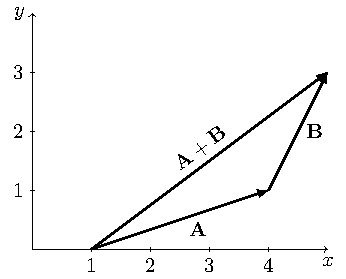
\includegraphics{figVectorHeadToTailRule}
\caption{سر کے ساتھ دُم جوڑ کر مجموعہ حاصل کیا جاتا ہے۔}
%\label{شکل_سمتیہ_سر_دم_جوڑنا}
\end{subfigure}
%
\begin{subfigure}{0.5\textwidth}
\centering
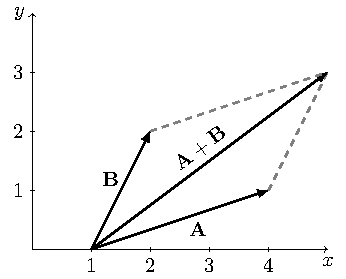
\includegraphics{figVectorParallelogramAdditionLaw}
\caption{متوازی الاضلاع سے بھی مجموعہ حاصل کیا جاتا ہے۔}
%\label{شکل_سمتیہ_متوازی_الاضلاع}
\end{subfigure}
\caption{سمتیوں کے مجموعے کا حصول}
\label{شکل_سمتیہ_سمتیوں_کا_مجموعہ}
\end{figure}

سمتیوں کے تفریق کا اصول  جمع کے اصول سے حاصل کیا جا سکتا ہے۔ہم $\bf{A}-\bf{B}$ کو $\bf{A}+\left(-\bf{B}\right)$ لکھ سکتے ہیں جہاں $-\bf{B}$ سے مراد یہ ہے کہ سمتیہ $\bf{B}$ کی سمت الٹی کر دی گئی ہے۔یوں $\bf{A}-\bf{B}$ حاصل کرنے کی خاطر $\bf{B}$ کی سمت الٹی کرتے ہوئے اس نئے سمتیہ کو $\bf{A}$ کے ساتھ جمع کیا جاتا ہے۔

سمتیہ \سمتیہ{A} کو مقداری \عددیء{k} سے ضرب دینے سے سمتیہ کی سمت پر کوئی اثر نہیں ہوتا جبکہ اس کی لمبائی \عددیء{k} گنا ہو جاتی ہے۔ 

\حصہ{کارتیسی محدد}
ایسا طریقہ جس سے کسی نقطے کا مقام بیان کیا جائے محدد\فرہنگ{محدد}\حاشیہب{coordinates}\فرہنگ{coordinates} کہلاتا ہے۔ہموار سطح پر کسی بھی نقطے کو دو محدد سے ظاہر کیا جا سکتا ہے۔خلاء تین طرفہ\حاشیہب{three dimensional} ہے لہٰذا خلاء میں کسی بھی نقطے کو تین محدد سے ظاہر کیا جا سکتا ہے۔شکل \حوالہ{شکل_سمتیہ_اکائی_سے_سمتیہ_کا_اظہار}-الف میں دو طرفہ  کارتیسی محدد پر اکائی لمبائی کے دو سمتیہ \سمتیہ{a_x} اور \سمتیہ{a_y} دکھائے گئے ہیں۔اکائی سمتیہ \سمتیہ{a_x} کی سمت مثبت \عددیء{x} جانب کو ہے جبکہ \سمتیہ{a_y}  کی سمت مثبت \عددیء{y} جانب کو ہے۔شکل-ب میں \سمتیہ{A} دکھایا گیا ہے۔کسی بھی سمتیہ کو دو یا دو سے زیادہ سمتیوں کے مجموعے کی شکل میں لکھا جا سکتا ہے۔شکل میں \سمتیہ{A} کو \سمتیہ{A_x} اور \سمتیہ{A_y} کے مجموعے کی شکل میں دکھایا گیا ہے یعنی
\begin{align}
\bf{A}=\bf{A_x}+\bf{A_y}
\end{align}

\begin{figure}
\begin{subfigure}{0.5\textwidth}
\centering
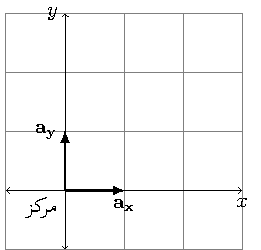
\includegraphics{unitVectorsInTwoDimensionalCartesianSpace}
\caption{اکائی سمتیہ}
%\label{شکل_سمتیہ_سر_دم_جوڑنا}
\end{subfigure}
%
\begin{subfigure}{0.5\textwidth}
\centering
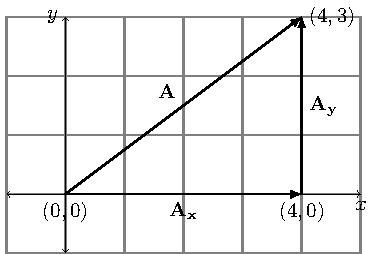
\includegraphics{vectorsRepresentationCartesianSpace}
\caption{اکائی سمتیوں کی مدد سے کسی بھی سمتیہ کو ظاہر کیا جا سکتا ہے۔}
%\label{شکل_سمتیہ_متوازی_الاضلاع}
\end{subfigure}
\caption{اکائی سمتیہ اور ان کا استعمال}
\label{شکل_سمتیہ_اکائی_سے_سمتیہ_کا_اظہار}
\end{figure}
%==================
\حصہ{سمتی رقبہ}\حاشیہط{اس کو باب کے آخر میں رکھنا ہے}
کسی بھی ہموار سمتی سطح کو سمتی رقبہ 
